\documentclass[11pt,a4paper,twoside]{article}

% LaTeX-Umsetzung der "Richtlinien für Projekt- und Diplomarbeiten"
% der LFE Medieninformatik, LMU München. (Autor: Richard Atterer, 27.9.2006, 23.10.2007), Bug-Fixing Mark Kaczkowski (23.6.2008)
\usepackage[backend=biber, style=ieee]{biblatex}
\usepackage{makecell}
\addbibresource{sample.bib}
\usepackage[T1]{fontenc} % sonst geht \hyphenation nicht mit Umlauten
\usepackage{booktabs}
\usepackage{listings}
%\usepackage[latin1]{inputenc} % man kann schreiben äöüß, statt "a"o"u"s
\usepackage[utf8]{inputenc} % wie oben, aber UTF-8 als Encoding statt ISO-8859-1 (latin1)
%\usepackage[ngerman,english]{babel} % deutsche Trennregeln, "Inhaltsverzeichnis" etc.
% \usepackage{ngerman} % Alternative zum Babel-Paket oben
% \usepackage{mathptmx} % Times-Roman-Schrift (auch für mathematische Formeln)
\usepackage{tgpagella}
% Zum Setzen von URLs
\usepackage{color}
\definecolor{darkred}{rgb}{.25,0,0}
\definecolor{darkgreen}{rgb}{0,.2,0}
\definecolor{darkmagenta}{rgb}{.2,0,.2}
\definecolor{darkcyan}{rgb}{0,.15,.15}
\usepackage[plainpages=false,bookmarks=true,bookmarksopen=true,colorlinks=true,
  linkcolor=darkred,citecolor=darkgreen,filecolor=darkmagenta,
  menucolor=darkred,urlcolor=darkcyan]{hyperref}
\usepackage{caption}
\usepackage{subcaption}

% pdflatex: Bilder in den Formaten .jpeg, .png und .pdf
% latex: Bilder im .eps-Format
\usepackage{graphicx}

\usepackage{subfiles}

\usepackage{fancyhdr} % Positionierung der Seitenzahlen
\fancyhead[LE,RO,LO,RE]{}
\fancyfoot[CE,CO,RE,LO]{}
\fancyfoot[LE,RO]{\Roman{page}}
\renewcommand{\headrulewidth}{0pt}
\setlength{\headheight}{13.6pt} % behebt headheight Warning

% Korrektes Format für Nummerierung von Abbildungen (figure) und
% Tabellen (table): <Kapitelnummer>.<Abbildungsnummer>
\makeatletter
\@addtoreset{figure}{section}
\renewcommand{\thefigure}{\thesection.\arabic{figure}}
\@addtoreset{table}{section}
\renewcommand{\thetable}{\thesection.\arabic{table}}
\makeatother

\sloppy % Damit LaTeX nicht so viel über "overfull hbox" u.Ä. meckert

% Ränder
\addtolength{\topmargin}{-16mm}
\setlength{\oddsidemargin}{25mm}
\setlength{\evensidemargin}{35mm}
\addtolength{\oddsidemargin}{-1in}
\addtolength{\evensidemargin}{-1in}
\setlength{\textwidth}{15cm}
\addtolength{\textheight}{34mm}
%______________________________________________________________________

\begin{document}

\pagestyle{empty} % Vorerst keine Seitenzahlen
\pagenumbering{alph} % Unsichtbare alphabetische Nummerierung

\begin{center}
\textsc{Ludwig-Maximilians-Universität München}\\
Department ``Institut für Informatik''\\
Lehr- und Forschungseinheit Medieninformatik\\
Prof.\ Dr.\ Heinrich Hußmann

\vspace{5cm}
{\large\textbf{Masterarbeit}}\vspace{.5cm}

{\LARGE Increasing Robustness of Facial Expression Recognition against Speech}\vspace{1cm}

{\large Marcel Baur}\\\href{mailto:marcel.baur@campus.lmu.de}{marcel.baur@campus.lmu.de}

\end{center}
\vfill

\begin{tabular}{ll}
Bearbeitungszeitraum: & 1. 1. 2021 bis 2. 7. 2021\\
Betreuer: & Matthias Schmidmaier\\
Externer Betreuer: & Ciprian Corneanu\\
Verantw. Hochschullehrer: & Prof. Hußmann
\end{tabular}
%______________________________________________________________________

\clearpage
% \section*{Zusammenfassung}

% Kurzzusammenfassung der Arbeit, maximal 250 Wörter.

% \selectlanguage{english}
\section*{Abstract}

Short abstract of the work, maximum of 250 words.

% \selectlanguage{ngerman}
\clearpage
\section*{Aufgabenstellung}

Kopie der Original-Aufgabenstellung

\vfill % Sorgt dafür, dass das Folgende an das Seitenende rutscht

\noindent Ich erkläre hiermit, dass ich die vorliegende Arbeit
selbstständig angefertigt, alle Zitate als solche kenntlich gemacht
sowie alle benutzten Quellen und Hilfsmittel angegeben habe.

\bigskip\noindent München, 02.07.2021

\vspace{4ex}\noindent\makebox[7cm]{\dotfill}

%______________________________________________________________________

\cleardoublepage
\pagestyle{fancy}
\pagenumbering{roman} % Römische Seitenzahlen
\setcounter{page}{1}

% Inhaltsverzeichnis erzeugen
\tableofcontents

%Abbildungsverzeichnis erzeugen - normalerweise nicht nötig
%\cleardoublepage
%\listoffigures
%______________________________________________________________________

\cleardoublepage

% Arabische Seitenzahlen
\pagenumbering{arabic}
\setcounter{page}{1}
% Geändertes Format für Seitenränder, arabische Seitenzahlen
\fancyhead[LE,RO]{\rightmark}
\fancyhead[LO,RE]{\leftmark}
\fancyfoot[LE,RO]{\thepage}

% \chapter{Introduction}
\section{Introduction}

Recognising facial expressions and the underlying emotions is important for human interaction. Through those facial expressions humans can detect and sense the underlying emotional state of their peers, playing a vital part in social discourse. The ability to recognise facial expressions artificially opens up many applications in human-computer interaction, like market research and content evaluation.

A key figure in the study of human emotion and its perception through facial expressions was Paul Ekman \cite{ekman1987universals} \cite{ekman1992basic} \cite{ekman2013emotion}. The focus of his work was to demonstrate that emotions express themselves universally in facial expressions, and are discrete classes of a emotional set \cite{ekman1987universals}.

Going forward several years into the mid-90s, Picard consolidated ideas of computing and measuring affect as a field of computer science in her 1995 essay, coining the term Affective Computing \cite{picard2000affective}. A subfield of affective computing is based around recognising affective states from facial expressions by combining advancements in computational ability with the research of Ekman \cite{ekman1987universals} \cite{friesen1978facial} and Russell \cite{russell1980circumplex}. Much of the progress in this field bases its research around several axiomatic assumptions, one of which being that all facial movements are induced by emotion. This is especially problematic if the analysed subject is speaking, since the act of talking also triggers facial movement and thus introduces noise into the input data. An example of this can be seen in figure \ref{fig:mislabel}. 

In this thesis, we explore ways to make facial expression recognition models more robust against speech. We analyse ability of humans to detect and judge facial expressions on talking subjects. To explore this we organised data collection and annotators using a web tool to label parts of an existing dataset (Section \ref{sec:human}). This suggested that \textit{humans are more accurate in judging emotions when confronted with a video instead of single frames}. Humans also were \textit{consistent in regards to the lexical content of the video}, being equally accurate no matter what was being said.

In section \ref{sec:models} we build on the insights from section \ref{sec:human} in two main ways to increase the robustness of facial expression recognition against speech:

\begin{enumerate}
    \item The addition of a \textbf{temporal dimension}: Speech is inherently temporal. We want to utilise this and leverage the contextual nature of the facial movements that relate to speech through temporal compensation.
    \item The inclusion of a \textbf{lexical compensator}: By including lexical compensators, we want to separate facial movements induced by speech from those that are induced by emotion and thus increase the robustness of our models against speech.
\end{enumerate}

We adopt state-of-the-art recurrent deep neural networks to add a temporal dynamic to our network, estimating the emotion over a given time instead of a frame by frame approach of classic facial expression recognition models. Lexical compensators are introduced as separate models that will produce additional inputs for our facial expression recognition model. We follow two approaches from previous work \cite{bursic2020improving} \cite{salman2020style}, and try to build on those. We end up with three different models:

\begin{itemize}
    \item Temporal facial expression recognition model
    \item Temporal facial expression recognition model including LipNet, a model specifically trained for lipreading, as a lexical compensator \cite{bursic2020improving}
    \item Temporal facial expression recognition model including a self-trained style extractor as a lexical compensator \cite{salman2020style}
\end{itemize}

To further analyse our models, we will validate them on separate datasets. One of those datasets will be in German to analyse the impact of a different language to the one used in the training dataset. Details on how we collected the data and the resulting analysis can be found in section \ref{sec:data}.

We conclude that the \textit{temporal compensation is the main factor in creating facial expression recognition models that are robust against speech}. Our experiments in sections \ref{sec:model_results} and \ref{sec:data_discussion} show an increase in performance with more temporal information. \textit{Models with lexical compensation show promise}, but do not significantly outperform models without it in its present state.

\begin{figure}
    \centering
    \includegraphics[width=0.8\textwidth]{res/png_backup/mislabel.png}
    \caption{An example of a model automatically predicting emotions from the face of a speaking subject while expressing a \texttt{sad} emotion \cite{livingstone2018ryerson}. Ideally, all frames would be correctly categorized as \texttt{sad}. Because of facial movements related to speech, the model only predicts the correct emotion twice. In this thesis we will work on creating models that are robust against predicting emotions from speaking subjects.}
    \label{fig:mislabel}
\end{figure}
\section{Background and Related Work}
\label{sec:related}

\subsection{Artificial Intelligence Techniques - Neural Networks}
\label{sub:aiml}
In this section we will describe common Artificial Intelligence (AI) techniques used in models for  facial expression recognition (Section \ref{sub:rw_fer}).
\subsubsection{Neural Networks}
A \emph{Neural Network NN} is built as a network with many \emph{neurons}, which are connected by \emph{activators} that have a \emph{weight}. These neurons are located in many layers which give structure to the NN \cite{schmidhuber2015deep}. The first layer of the NN is the so-called \emph{input layer}, which acts as the entry point for the data that is to be analysed. The last layer is defined as the \emph{output layer}. It contains the information about the estimation that the NN has made. The in-between layers are called \emph{hidden layers}.

More formally, each output of a neuron can be written as a function:

\begin{equation}
    h_i = \sigma (\sum_{j=1}^{N} w_{ij}x_{j})
\end{equation}

The function $\sigma$ describes the activation, $N$ the amount of neurons that are the input to the current neuron. The weight of the input connection from each neuron of the previous layer is described by $w$.

Activation functions can introduce non-linearity to a network. They can also bound the final value of an activation in a specific range to combat divergent neurons which may paralyze the NN \cite{wang2003artificial}. They also provide stability in gradient-based learning.
\bgroup
\def\arraystretch{2}
\begin{table}[]
    \centering
    \begin{tabular}{l|c|c}
        \textbf{Activation Function} & \textbf{Equation} & \textbf{Range} \\ \hline \hline
         Sigmoid & $\frac{1}{1 + e^{-x}}$ &  $(0,1)$\\\hline
         Softmax & $\frac{e^{x_i}}{\sum_{j=1}^{J} e^{x_i}}$ & $(0,1)$\\\hline
         ReLU & $max(0, x)$ & $[0, \infty]$ \\\hline
         Tanh & $\frac{e^x - e^{-x}}{e^x + e^{-x}}$ & $(-1, 1)$\\\hline
    \end{tabular}
    \caption{An overview of selected activation functions which we will use in our models (Section \ref{sec:models})}
    \label{tab:my_label}
\end{table}
\egroup

A NN can also be represented as a very complex function $f(x) = y$, where $x$ represents the input, and $y$ the computed output (the prediction).

Shallow NN consist of few hidden layers, and have been a topic for a long time. The discovery of \emph{backpropagation} allowed the development of NNs with many hidden layers, called \emph{Deep Neural Networks DNN} \cite{schmidhuber2015deep}.

\subsubsection{Convolutional Neural Networks CNN}
CNNs lend themselves well to tasks in \emph{Computer Vision CV} \cite{albawi2017understanding}. Most importantly, they reduce the amount of parameters, while also emphasizing locality and context of the input information. This enables edge detection, shape detection, and object detection in successive layers of a deep CNN, which will be especially helpful in models (Section \ref{sec:models}) that analyse faces and their active Action Units (Section \ref{subsub:au}).

Subsequent convolutional layers, coupled with pooling layers, enable the detection of more and more complex structures. While the initial layers might detect straight edges, the following layers will recognize compound structures, and ultimately features like raised eyebrows (AU 1 and/or AU 2).

\paragraph{Convolution}
The convolutional layers in a CNN provide locality and size reduction to the network. Since we work with image inputs in our thesis, we will provide such an example here.

Consider a greyscale image of a face with a width and height of 256x256 pixels. Each pixel is represented by a single greyscale value, putting the dimensionality of the image at 256x256x1. Layering this input image with a traditional dense layer of size 10 would already produce $256 \cdot 256 \cdot 10 = 655360$ weights that have to be trained. 

A (in this case two dimensional) convolutional layer only looks in local regions of the image to produce an output to the next layer. A sliding window of $n$ x $m$ pixels will scan the input image in a set stride, and produce values for the next layer with substantially less weights attached. Pre-set windows (also called matrices) of size 3 x 3 can be used to detect edges in images, or transform them with sharpening or blurring effects.

\paragraph{Pooling}
Pooling layers are used to decrease the size of the layers and create a more efficient embedding. A window of size $n$ x $m$ slides across the layer again, this time only producing a single value for each step. A common technique is to select the largest value in the current window, creating a so-called \emph{MaxPooling} layer. Figure \ref{fig:pooling} shows a MaxPooling layer working on a 4 x 4 matrix.

\begin{figure}
    \centering
    \includegraphics{res/pooling.pdf}
    \caption{An example of a MaxPooling layer working on the left matrix with a window size of 2 x 2 and a stride of 2, producing the matrix on the right.}
    \label{fig:pooling}
\end{figure}

\subsubsection{Temporal Neural Networks with Gated Recurrent Units GRU}
The previously described NNs can be described as \emph{feedforward} NNs. The direction of information flow is linearly through input, hidden and to the output layer. This can be contrasted with \emph{feedback} NNs, that have mechanisms that allow for 'memory' in a NN \cite{wang2003artificial}. These \emph{Recurrent Neural Networks RNN} enable the analysis of temporal data.

A concrete implementation for a temporal recurrent layer are \emph{Gated Recurrent Units GRU} proposed by Cho et al. \cite{cho2014properties} \cite{chung2014empirical}. GRUs act similarly to \emph{Long Short Term Memory LSTM} \cite{hochreiter1997lstm} layers, while removing memory gates \cite{chung2014empirical}. Empirical research has shown that GRUs can be more performant than LSTMs in less frequent datasets \cite{gruber2020gru}.


\subsubsection{Architectures}
NNs can be built in various different ways. Over time, researchers have developed predifined structures of NNs which are reused for many different applicaitons. These different structures are more commonly referred to as \emph{architecutres}. In this thesis we will come across the two well known architectures \emph{VGG} and \emph{MobileNet}.
\paragraph{VGG}
Introduced by Simonyan and Zisserman in 2014 \cite{simonyan2015vgg}, VGG16 and VGG19 have established themselves as architectures for image classification, including facial expression recognition. VGG16 achieved top-5 finishes in the 2014 ImageNet Challenge in both localisation and classification tasks. A major drawback to models using the VGG architecture is its computing performance. Given its rather large architecture, it is comparatively slow to train. This is where we turn to \emph{MobileNets}.
\paragraph{MobileNet}
\emph{MobileNets} were originally introduced for mobile and embedded vision applications \cite{howard2017mobilenets}. They allow for hyperparameter tuning, where the developer is able to choose a fitting model size for his application based on two global hyperparameters. MobileNets trade off accuracy (and thus the need for many hidden layers) in favour of speed and efficiency. Our core facial expression recognition models are based on the MobileNet architecture.


\subsection{Emotional Models from Facial Expression}
\label{sub:rw_fer}
We now need a way to leverage the tools we mentioned above to build models that accurately estimate the affective state. Ekman, Russell, Posner and many others have developed systems that rigidly define the emotional state of a subject. While dimensional models, which define the affective state through several dimensions, we will focus on the \emph{categorical model} that works on emotional classes. 

\paragraph{Categorical Model}
One of the most recognized ways to separate emotional states in non-verbal communication is presented by Paul Ekman \cite{ekman1987universals} \cite{ekman2013emotion}. His research postulates a cross-cultural agreement in judging facial expressions \cite{ekman1987universals}. Basic emotion theory assumes a fixed amount of human emotions, which is also believed and postulated by Ekman and Russell \cite{ekman1992basic} \cite{russell2006}. Ekman proposes a split into seven categories: anger, happiness, surprise, sadness, fear, disgust and contempt. He later consolidated them down to six, removing contempt. 

% \subsubsection{Dimensional Model}

% Dimensional systems use a set of dimensions, \emph{valence}, \emph{arousal} and in some cases \emph{dominance} to estimate the affective state of a person. James A. Russell introduced the two dimensional circumplex model of affect \cite{russell1980circumplex}, where he mapped emotions in the valence-arousal space. Valence represents the (un-)pleasantness of an affective state, and arousal represents the activation. \cite{posner2005circumplex}. The emotions from the categorical have their place in this dimensional field, e.g. happy having a high score for valence and arousal.

% \begin{figure}
%     \centering
%     \includegraphics[width=0.8\textwidth]{res/circumplex.png}
%     \caption{The circumplex model of affect with the valence and arousal axis with selected emotions. \cite{russell1980circumplex} \cite{pourmirzaei2021an}}
%     \label{fig:circumplexImg}
% \end{figure}

\subsubsection{Action Units}
\label{subsub:au}

Introduced by Hjortsjö \cite{hjortsjo1969man} and further refined by Ekman \cite{friesen1978facial}, the \emph{Facial Action Coding System FACS} tries to separate and classify facial movements that lead to distinct facial expressions. Combinations of the 28 \emph{Action Units AUs} can then be used to describe an affective expression.

\begin{table}[]
    \centering
    \begin{tabular}{c|c}
       \textbf{Emotion}  & \textbf{Action Units} \\ \hline
        Happy & 12, 25 \\
        Sad & 4, 15 \\
        Fearful & 1, 4, 20, 25 \\
        Angry & 4, 7, 24 \\
        Surprised & 1, 2, 25, 26 \\
        Disgusted & 9, 10, 17
    \end{tabular}
    \caption{The basic emotions with their corresponding prototypical AUs \cite{fabian2016emotionet}}
    \label{tab:emotionAUs}
\end{table}

\subsection{Automatic Facial Emotion Recognition}
Facial Emotion Recognition FER can be divided into two different groups: conventional and Deep-Learning-based. \cite{ko2018brief}

Conventional FER systems work in a pipeline that consists of three steps: face detection, feature extraction and expression classification. The first step crops the input image to the face to ignore unneccesary input information. Facial landmarks can at times also be detected here. The second step detects features based on the data extracted from the previous step. Those features then are used to classify an emotion for the input \cite{ko2018brief}.

The deep learning approach has established itself as the state-of-the-art method for FER models. In contrast to the handcrafted conventional pipeline, the more modern approach enables an end-to-end learning method \cite{ko2018brief}. The most prominent model-type in FER is the convolutional neural network CNN. CNN-based networks offer themselves very well to image processing, which make them a great candidate for FER systems. 

Deep learning models can further be divided into two categories. The first one outputs emotions directly from the model \cite{ebrahimi2015recurrent} \cite{kim2017multi} \cite{jung2015joint}, where the second one classifies AU activations, from which emotions can be deduced \cite{breuer2017deep} \cite{zhao2016deep} \cite{chu2017learning}. 

\begin{figure}
    \centering
    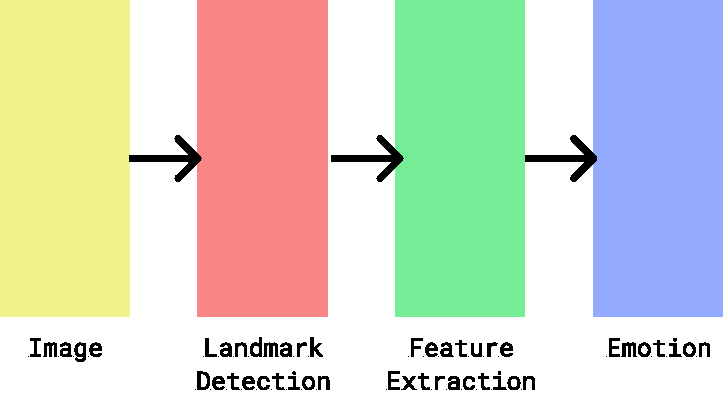
\includegraphics[width=0.8\textwidth]{res/PipelinePrototype.pdf}
    \caption{PROTOTYPE: An example of a FER pipeline. After extracting landmarks from the target image, models try to extract features from the given landmarks. These can be used to detect an emotion from the input.}
    \label{fig:pipeline_fer}
\end{figure}

\subsection{Phonemes and Visemes}
The content of an act of speech can be segmented into words, syllables, and \emph{phonemes} \cite{savin1970nonperceptual}. Languages differ in their amount of phonemes, with the New Guinean language Rotokas having 11, whereas the Namibias !Xóõ is using 160. English, the primary language we're be looking at in this thesis, has 37-41 phonemes, differing by dialect \cite{Hayes2009}. Phonemes are very important in FER. A speaking subjects face, and activated AUs, will be influenced by the lexical content of their speech, which is defined by the current phoneme. The face of a person in the act of pronouncing a phoneme will have a certain look to it. Several phonemes can be grouped together based on the distinct look they produce. These groups are called \emph{visemes}. There are several different phoneme-to-viseme mappings in research, with no concrete agreement on a 'best mapping' \cite{cappelletta2012viseme}.

Visemes are particularly interesting for us, since our research is purely based in the visual domain. Differences between phonemes that are purely audiocentric are of no relevance for us. A viseme mapping reduces the categories for visually based lexical content, which makes building and training models easier.

\begin{figure}
    \centering
    \includegraphics[width=0.8\textwidth]{res/phoneme.png}
    \caption{A visual example of three phonemes being spoken, together with their occurrence in a sentence.}
    \label{fig:phoneme_ex}
\end{figure}

\subsubsection{LipNet}

LipNet is an end-to-end sentence-level lipreading model that is based on visual data \cite{assael2016lipnet}. It specifically is not based on word classification, the authors stress the sentence-level lipreading comprehension. It operates on the character-level, combining CNNs with RNNs.

\begin{figure}
    \centering
    \includegraphics[width=0.8\textwidth]{res/lipnet.png}
    \caption{The architecture of LipNet \cite{assael2016lipnet}. A batch of \textit{t} frames is fed into the network. A combination of Spatio-Temporal CNN layers with Spatial Pooling layers feed into two GRUs.}
    \label{fig:lipnet}
\end{figure}

The LipNet model is trained on the GRID corpus \cite{cooke2006grid}, where it achieves a 95.2\% sentence-level word accuracy.

The input of the model is a cropped region around the orofacial area of the face. The dimension of this region is set to 100x50 pixels, and the default frame batch size is set to 75 frames.

We will use an embedding of LipNet in one of our models to create a lexical compensator.

\subsubsection{FaceMesh}


FaceMesh is a model to create 3-dimensional models of the facial surface geometry in real time videos \cite{kartynnik2019facemesh}. It creates 468 3-dimensional landmark points on the face, which are arranged in fixed quads.

\begin{figure}
    \centering
    \includegraphics[width=0.5\textwidth]{res/facemesh2.png}
    \caption{The mesh topology of FaceMesh. The 468 landmark points are projected on a screen. Neighbouring points are connected to form three-sided polygons.}
    \label{fig:facemesh}
\end{figure}

FaceMesh was originally implemented in tensorflow.js, making it only available on JavaScript runtimes. The mediapipe project published a port to a Python implementation, which we used of our models.

The model was trained on around 30,000 diverse, in-the-wild images which were also augmented while training. Annotating the images was done in an iterative approach \cite{kartynnik2019facemesh}:
\begin{enumerate}
    \item Initial model in supervised approach through synthetic renderings of 3D morphable models or 2D landmarks from annotated in-the-wild images.
    \item Refine the x- and y-coordinates by using the latest model while filtering out predictions where the prediction error is tolerable. Other predictions were improved through annotation.
\end{enumerate}
\subsubsection{Montreal Forced Aligner}
\label{sub:mfa}
The Montreal Forced Aligner MFA is an open source software for speech-text alignment \cite{mcauliffe2017montreal}. A forced aligner is a tool that aligns speech and it's corresponding transcription on a word and phone level. This allows for precise estimations of phoneme occurrence in audio files.

The MFA builds on Kaldi \cite{povey2011kaldi}, a speech recognition toolkit which allows for easy distribution due to Kaldi's open-source license.

We will use the MFA to align our datasets and to get a precise phoneme-to-video mapping, enabling us to extract frames where specific phonemes were said by the actors.

\begin{figure}
    \centering
    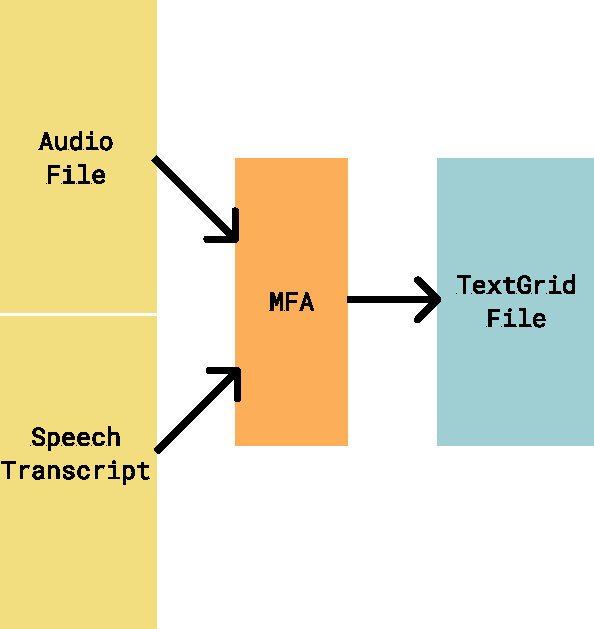
\includegraphics[width=0.5\textwidth]{res/mfa.pdf}
    \caption{A pipeline of a classic use of the MFA. An audio file, together with its transcript gets fed into the MFA. The output of the aligner is a \texttt{TextGrid} file that contains timestamp information about word and phoneme occurrence in the input audio file.}
    \label{fig:mfa}
\end{figure}
\subsection{Existing Approaches to Compensate Speech Effects}
\label{sec:existing}
There have already been advances in FER that accounts for speech. In this section, we will present three models that will be relevant to our work.

\subsubsection{Blind Lexical Compensation}
Mariooryad and Busso \cite{mariooryad2015facial} propose a model that bases itself on a previous study, stating that facial expressions are the result of three factors that influence facial behaviours:

\begin{enumerate}
    \item The individual features and habits of the speaker
    \item The lexical content of the speech act
    \item The current affective state/emotion of the subject
\end{enumerate}

Their analysis also showed that "constraining the model on the lexical content makes the emotion variability the dominant factor in the mouth area" \cite{mariooryad2015facial} \cite{mariooryad2012factorizing}.

The authors aim to build a model using blind lexical compensation, a method that will not require a transcription of the lexical content. Their approach builds on the asymmetric bilinear model \cite{tenenbaum1997separating} \cite{tenenbaum2000separating}. This model aims to separate style from content. In this case, the style represents the emotion and the individual phoneme the content.

After training, the model consists of $N$ style matrices (with $N$ being the amount of emotions). Each style matrix represents an embedding for the corresponding emotion. To classify an input sample, the \emph{Expectation Maximization EM} algorithm was used, to achieve a soft assignment $p(s^{*}, c |y)$ (the probability of the sample $y$ belonging to style $s^{*}$ and content $c$.

After 10 EM cycles, a style matrix $A^{*}$ will be produced. The emotion estimation is done by calculating the frobenius norms to each trained style matrix, and using the label of the style matrix with the lowest distance.

Given that this approach requires facial landmarks and artificial mesh alrorithms were not as established at the time, the dataset of choice was IEMOCAP. This leads to the model only having four classes (Happiness, Anger, Sadness, Neutrality).

\subsubsection{Lexical Compensation with LipNet}
Bursic et al. \cite{bursic2020improving} created a NN centered around lexical compensation using LipNet. While they present several approaches in their paper, we are most interested in their Lip Model, which is build by merging a LipNet embedding with an embedding of a classic VGG19 FER model. The models have also been temporalized, with several different frame batches ranging from 5 to 65 frames. Their best performing Lip Model was set at 60 frames per prediction, reaching an accuracy of 59.4\%. In comparison, the face-only RNN model that does not include lexical compensation from LipNet reached it's best accuracy at 40 frames and 48.5\%.

The dataset used in this paper was RAVDESS, using the core emotions from Ekman, ignoring \emph{calm}. This makes for a good comparison to our models.

We will compare our experiments of using LipNet as a lexical compensator their results in section \ref{sec:models}.

\begin{figure}
    \centering
    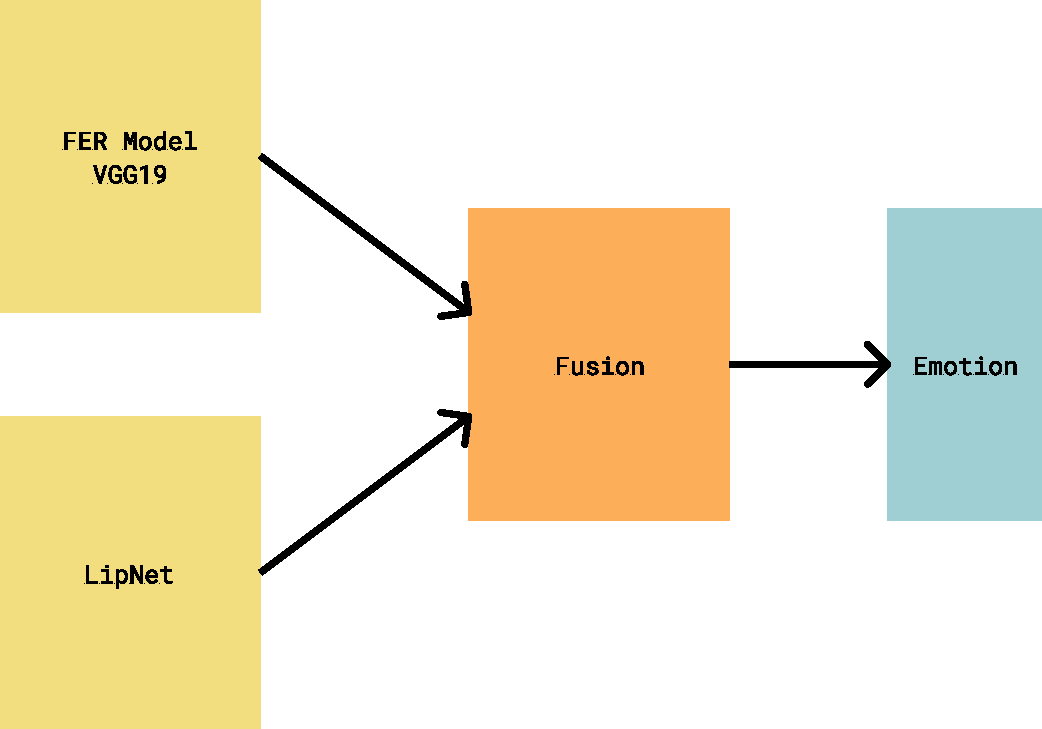
\includegraphics[width=0.8\textwidth]{res/bursicschema.pdf}
    \caption{The schema of the Lip RNN by Bursic et al. \cite{bursic2020improving}.}
    \label{fig:bursic_schema}
\end{figure}

\subsubsection{Lexical Compensation using a Style Extractor}
Salman and Busso \cite{salman2020style} have a similar approach to Bursic, using a lexical compensator alongside a feature extractor with an embedding of a classic FER model using the VGG16 architecture.

The major point of interest is their style extractor/lexical compensator (see Figure \ref{fig:bussose}). It uses facial meshes of the subject instead of images, generalizing it against the subject. The model is trained on a temporal NN with one input and two outputs: an emotional mesh of a face serves as the input, producing a neutral mesh alongside a phoneme prediction. The idea is that the difference between the emotional input mesh and the neutral output mesh can give us information about the facial movements that are produced by emotional activations.

We will use a similar feature extractor in our experiments. Since Salman and Busso only trained their model on four emotions, comparisons will be challenging. We will rather compare our results with the performance of our other models, trying to determine the impact of the lexical compensator that way. 

\begin{figure}
    \centering
    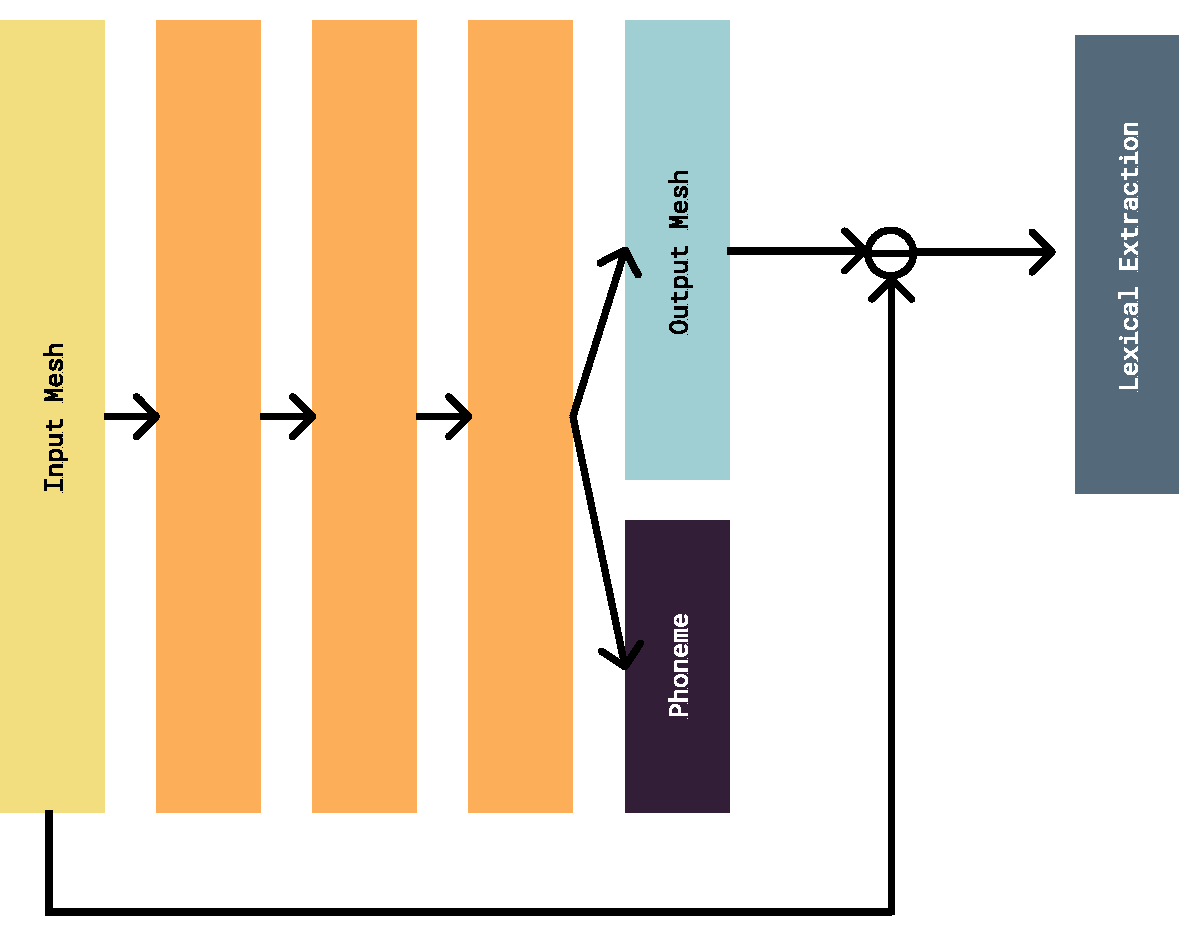
\includegraphics[width=0.8\textwidth]{res/BussoSE.pdf}
    \caption{The schemal of Salman and Busso's lexical compensator. An emotional mesh is the input to a NN, producing a neutral output mesh alongside a phoneme prediction. The difference of the input mesh and the output mesh extracts the facial movements that are produced by the emotional state of the subject.}
    \label{fig:bussose}
\end{figure}

\subsubsection{Temporal Compensation}
The previous two models both used a temporal approach alongside their efforts of lexical compensation. Opposed to the more traditional way of FER where only single images were classified, a temporal model estimates the emotion on a sequence of images. 


\subsection{Datasets}

\subsubsection{AffectNet}
\emph{AffectNet} is one of the largest image databases for affect. It consists of around 450,000 manually annotated images. Labellers classified them by eight emotional categories (Neutral, Happy, Sad, Surprise, Fear, Anger, Disgust, Contempt) while also providing continuous labels for valence and arousal. In addition to the labelled images, 1,000,000 images with facial landmarks are provided.

The images were collected by scraping the internet through querying various search engines. Faces were recognized with the \emph{OpenCV} toolkit. Facial landmarks were extracted with regression of binary features \cite{ren2014face}.

Labelling the 450,000 images was done by 12 full-time and part-time annotators who were knowledgeable on the issues of emotion and affect, and were specifically hired for the task. This was done to remove the issue of low-quality labels that occur with crowd-sourced methods. \cite{mollahosseini2017affectnet}

Our classic FER models we will use are all trained on AffectNet.

\subsubsection{RAVDESS}
\label{sub:ravdess}
The Ryerson Audio-Visual Database of Emotional Speech and Song (RAVDESS) is a validated multimodal database for emotional analysis \cite{livingstone2018ryerson}. It contains videos of speech and song from 24 professional actors. The database is gender balanced, and the actors were chosen with the ability of speaking a neutral North American accent. The database contains videos in eight emotions (Calm, Happy, Sad, Angry, Fearful, Surprise, Disgust, Neutral) in the speech acts, which are the important ones for us.

The actors were tasked with speaking two pre-defined sentences ("Dogs are sitting by the door", "Kids are talking by the door") in the given emotions, across two levels of intensity. Across all actors, 1440 audio-visual files of speech acts were recorded. Audio- and video-only files are provided as well.

RAVDESS lends itself very well to our research by including all core emotions and providing high quality footage. It also standardizes statements and lexical content, which lowers the amount of external factors that could influence our analysis and training. We focus our attention to the core emotions that are described by Ekman, which means that we ignored the videos for the calm emotion.

\begin{figure}
    \centering
    \includegraphics[width=0.8\textwidth]{res/img_ravdess_example_neutral_14AY1.png}
    \caption{A frame of a video from the RAVDESS database \cite{livingstone2018ryerson}. Actor 14 is pronouncing the phoneme \texttt{AY1} in a neutral emotion.}
    \label{fig:ravdess_example}
\end{figure}

\subsubsection{CREMA-D}
The Crowd-sourced Emotional Multi-modal Actors Database (CREMA-D) is a labelled multimodal for emotional analysis \cite{cao2014crema}. It contains 7,442 videos of speech acts from 91 actors of varying age and ethnicity. The database includes videos across seven emotions (Calm, Happy, Sad, Angry, Fearful, Disgust, Neutral) with scaled intensities. Surprised is notably missing from the emotional categories. The authors state that "surprise was not considered by the acting directors to be sufficiently specific, as it could relate to any of the other emotions with rapid onset" \cite{cao2014crema}. 

The authors also provided the individual ratings for each video, which were collected from 2,443 crowd-sourced raters. These can also be used to analyse human bias in emotion recognition (see Section \ref{sec:human}).

\subsubsection{MSP-IMPROV}
MSP-IMPROV is an acted multimodal database for emotional analysis \cite{busso2016msp}. It covers four emotions (Anger, Happiness, Sadness, Neutral), where twelce actors (6 male, 6 female) were tasked to speak 15 different statements. While recording, the actors were set in different scenarios, in which the target sentences were included. Only the target sentence had to be spoken word-for-word, the buildup to the scenario was open to improvisation.

652 recordings are provided on the target sentences. The authors also provide the statements on the entire improvised session, where 4,381 speaking turns are collected. 2,785 speaking turns were collected on natural interactions, where the actors were speaking normally to each other, outside of a scripted or improvised session. 620 turns were recorded on the target sentences alone, where the actors were tasked to read the statements in the provided emotion. This sums up the size of the MSP-IMPROV corpus to 7,818 recordings. 

\subsubsection{IEMOCAP}
The interactive emotional dyadic motion capture database (IEMOCAP) \cite{busso2008iemocap} is a labelled database based on dyadic interaction where one of the subjects is set up with motion capture software on their head, face and wrists. It is based on two types of interactions, acted and improvised.

The database is gender balanced, with 5 male and female actors each. The actors were students from the Drama Department of the University of Southern California.

The data was annotated by USC students. They labelled the utterances based on categorical expression (Neutral, Happiness, Sadness, Anger, Surprise, Fear, Disgust, Frustration, Excited, Other) and dimensional values for activation, valence, and dominance.

In total, 5,255 scripted turns and 4,784 improvised turns were recorded. 

\begin{figure}
    \centering
    \includegraphics[width=0.8\textwidth]{res/iemocap.png}
    \caption{The motion capture points of IEMOCAP. They cover 53 points on the face, a wristband with two markers, one marker for each hand, and a headband with two markers. \cite{busso2008iemocap}}
    \label{fig:iemocap_cap}
\end{figure}

% \chapter{Research}
\section{Human Labelling}
\label{sec:human}
\newpage
\section{Advancing Existing FER Approaches}
\label{sec:models}

In the previous section \ref{sec:human} we concluded that a temporal dimension, and a lexical compensator might help in improving existing FER models for speaking subjects. 

We will discuss temporal compensation in section \ref{sub:temp}. A lexical compensator will have to be done with a separate model. There are different approaches to this, as we have seen in section \ref{sec:existing}. We will discuss this in section \ref{sub:lex}.

\subsection{Temporal Compensation}
\label{sub:temp}
As discussed previously, we want to keep and build on existing FER models. Given that some of our models will work on video data, we will have to temporalize our models which currently work on static images.

The straight forward approach is to take the current model, and wrap it in a temporal layer. This means that an input video with 60 frames will produce 60 output embeddings (Figure \ref{fig:temporalization}), which can then be fed into a recurrent layer like a LSTM or GRU. This produces minimal overhead, while preserving all weights from our model.

We will use this approach in all our upcoming models.

To have a comparison between frame sizes and an estimation of the importance of the temporal dimension, our models were trained on 1, 30, 60, and 90 frames.

\begin{figure}
    \centering
    \includegraphics[width=0.8\textwidth]{res/png_backup/temporalisation.png}
    \caption{Temporalizing an FER model. The existing model gets wrapped in a TimeDimensional layer. That way the model produces $n$ embeddings for $n$ inputs.}
    \label{fig:temporalization}
\end{figure}

\subsection{Lexical Compensators}
\label{sub:lex}
We have presented two approaches to lexical compensation in sections \ref{sub:lip} and \ref{sub:style}. We will focus on those two previously mentioned approaches from Bursic \cite{bursic2020improving} and Busso \cite{salman2020style}, which attempt to extract lexical information in different ways. The goal of a lexical compensator is to extract the facial movements from speech to filter them out and extract the facial movements that are induced by the subjects emotional state.

\paragraph{LipNet} 
Bursic et al. \cite{bursic2020improving} used a LipNet embedding to detect the lexical content. We reproduced their approach to analyse the performance of the architecture, using our own MobileNet. The dataset of choice, similarly to the original model, was RAVDESS. The validation data consisted of all the recordings of actors 4 and 5.

As we have seen in section \ref{sec:lipnet_related}, LipNet requires a orofacial crop of size 100x50. A sequence of frames are passed into the network, which then gets analysed by GRU layers after a set of convolutions and poolings (Figure \ref{fig:lipnet}). We cut the network after the three layers of convolution and spatial pooling to yield an embedding for every frame. The output of the last pooling layer has a dimensionality of 96x3x6, which we passed to another MaxPooling layer of size 1x6x3 and stride 1x1x1 to create a flattended vector with 92 values and make it compatible with the concatenate step described in section \ref{sec:building}. This embedding gives us an indication of the features in the orofacial region, where the majority of lexical information in a visual feature space resides \cite{mariooryad2012factorizing}. The models then can compensate for the lexical content using this embedding.

\paragraph{Style Extractor}
The core idea of a style extractor is to separate the style (emotion) from the content (sentence/words/phonemes). Attempts at this have been published by Salman and Busso \cite{salman2020style}. This type of lexical compensator served as the inspiration for our own. We made the following changes to the architecture and preprocessing of the style extractor: we turned to FaceMesh as a facial landmark detector, yielding 468 three-dimensional coordinates, 1404 inputs in total. Additionally, we chose a smaller, non-temporal architecture network, with only one hidden layer.

We trained different models to optimize the size of the style extractor. Given that a hidden layer of 3000 neurons overtrained the model, we stepped down to 512, 256, and 128 neurons. The validation loss of the model was chosen as the deciding metric. 
All three smaller models generalized well with a very similar validation loss. We ultimately continued with the smallest model, yielding a more compact model (Figure \ref{fig:fextractor}). A style extractor with a hidden layer of size 64 was not able to match the performance of the larger models, and exceeded the validation loss of the 128-sized model of 0.1048.

Another difference to the original approach was our decision to remove the second, unused output which predicts the underlying phoneme. Test runs using a phoneme output yielded no improvement on the actual style extractor output.

The dataset used to train this model, like in the original paper, was CREMA-D.

\begin{figure}
    \centering
    \includegraphics[width=0.5\textwidth]{res/png_backup/styleex.png}
    \caption{The architecture of our final feature extractor. The emotional input mesh of a subject speaking a given phoneme $p$ gets passed to a densely connected hidden layer with 128 neurons. The output of the network is a prediction of a neutral mesh of the actor pronouncing the same phoneme $p$.}
    \label{fig:fextractor}
\end{figure}

\subsection{Building the Models}
\label{sec:building}

To complete the architecture, we will briefly talk about the fusion layers. In instances where two model inputs come together (e.g. the lexical compensators) we need a network that combines both inputs. We want this fusion network to be consistent across all our models to make sure that differences in results are not due to differing architectures.

We turned to the fusion layer by Bursic et al. \cite{bursic2020improving}. We tried to replicate their approach with the lexical compensation from LipNet, and our FER model had a similar embedding with 512 neurons to their VGG19 model. This lets us better compare our results to theirs. In comparison to the model from Salman and Busso \cite{salman2020style}, this fusion network covers all seven core emotions.

To judge the impact of the lexical compensators we also trained a model that only uses the temporalized embedding of our FER model. We use the same fusion network, this time in a transfer learning approach. The FER embedding of 512 neurons gets passed to the same fusion network, foregoing the \texttt{concatenate} step. This aides in comparing the impact of the lexical compensators without having any noise from a differing transfer network.

The input from the previous model(s) are fed into a bidirectional GRU layer of size 256. A dense layer of size 16 follows. The final output layer is a densely connected layer of size 7, corresponding to the core emotions. The activation function of the hidden layers are ReLU, while the output layer has a softmax activation function. A dropout layer of 0.5 is placed between the GRU and the following dense layer (see Figure \ref{fig:fusionlayers}).

We end up with three main architectures, which we will train, validate, and compare:

\begin{enumerate}
    \item \textbf{Temporal FER model: FER-TC} The temporalized FER model without a lexical compensator, with 512 inputs.
    \item \textbf{Lexical compensation with LipNet: FER-LN} The temporalized FER model with LipNet as the lexical compensator, with 512 (FER) + 96 (LipNet) inputs.
    \item \textbf{Lexical compensation with our Style Extractor: FER-SE} The temporalized FER model with a self trained style extractor as the lexical compensator, with 512 (FER) + 1404 (Style Extractor) inputs.
\end{enumerate}

\begin{figure}
    \centering
    \includegraphics[width=0.7\textwidth]{res/png_backup/fusion.png}
    \caption{The architecture of the fusion/transfer network. It is kept simple to accommodate the smaller datasets we use and follows the architecture from Bursic et al. \cite{bursic2020improving}.}
    \label{fig:fusionlayers}
\end{figure}
\subsection{Data and Preprocessing}
\paragraph{Data for FER Models}
We mainly use two datasets in our work, RAVDESS and CREMA-D. Since the actual usage of the data is dependent on some common preprocessing steps like face-/mouth-cropping and landmark extraction, we transformed the datasets before starting training.

The FER-model takes a facial crop of the frame, with 224x224x3 dimensions (width, height, colour channels). The facial crop had to be proportional to the original image, so it was important not to stretch or morph the cropped frame (Figure \ref{fig:crop}). In preprocessing, we saved a crop of every frame for all videos. 
The LipNet model required a 100x50x3 dimensional input of the orofacial area. This crop was saved alongside the facial crop for each frame. Both the facial and orofacial crops were done with the frontal face detector of dlib \cite{dlib09}. Finally, our style extractor was be trained on facial landmarks extracted from FaceMesh. Those were also stored with the facial and orofacial crops.

Each videos data is saved as an array in a \texttt{pickle} file. The structure of the file can be seen in figure \ref{fig:pickle}.
\begin{figure}
    \centering
    \includegraphics[width=0.5\textwidth]{res/png_backup/pickle.png}
    \caption{The data structure of our preprocessed files. Each file corresponds to one video. Its facial and orofacial crops, alongside with its facial landmarks are stored in arrays. The array lengths correspond to the amount of frames in each video. The underlying emotion is saved as well.}
    \label{fig:pickle}
\end{figure}

\begin{figure}
    \centering
    \includegraphics[width=0.8\textwidth]{res/png_backup/crop.png}
    \caption{The input for the FER model had to be a crop of the subjects face, with a dimension of 244x244 pixels. It was important not to stretch the original crop and keep the proportions. We extended the facial bounding box to fit it to the required dimensions.}
    \label{fig:crop}
\end{figure}


\paragraph{Data for the Style Extractor}
To be able to train the style extractor we need pairs of meshes for every phoneme, where one mesh is emotional (not neutral) and one neutral. To have a more fine-grained model, we also made sure that all mesh pairs are from the same occurrence. As an example, the sentence "It's eleven \textbf{o}'cl\textbf{o}ck" has two occurrences of the phoneme \texttt{O} (marked). When training the style extractor, all mesh pairs came from the same actor in the same sentence from the same occurrence. We achieved this by using the MFA (see section \ref{sub:mfa}) to align the video files. Phonetic transcripts that do not have neutral counterparts were ignored. This left us with around 140.000 phoneme pairings to train the style extractor with. 


\subsection{Training}
Here we present more detailed information for the training process of our models, and discuss results from model validation.
\paragraph{General Information}
To keep the models comparable on the temporal dimension, we trained each model on 1, 30, 60, and 90 frames. The FER and LipNet model were pre-trained and frozen. We wanted to cover the core emotions that were defined by Ekman, and thus ignored the \texttt{calm} emotion that was provided by the RAVDESS dataset. Those files did not appear during training or validation and were discarded.

We used a sliding window approach on the frame arrays. Given a model with a frame size of 60 and a video with 100 frames, we now have the opportunity to extract multiple data point from the video. We used a window stride of 5. This means that the first data point ranges from frame 0 to 59, the second from 5 to 64 and so on. This helped to somewhat ease the problem of the RAVDESS dataset being too small for proper DNN training. 

Our specific style extractor was trained separately. It was trained on CREMA-D, with actors 1 to 11 being used for validation.

The fusion networks for all models was trained on RAVDESS. Actors 4 and 5 were used for the validation set, the files from the other 22 actors were used for training.

We used an early stopping and snapshot callback during training. If the validation loss dropped on three consecutive epochs, training was finished. The most accurate model on the validation set was saved and later used for further analysis in section \ref{sec:model_results}.

\paragraph{Technical Details}
We used the \texttt{keras} environment using a \texttt{tensorflow} backend (version 2.4.1) to train our models on a HPC using an Nvidia Titan X GPU with the Pascal architecture. The scripts were deployed in Docker containers, on a server running Ubuntu 18.04 LTS.

The preprocessed datasets were stored separately on the HPC and were injected into the docker container through virtual links. The \texttt{Dockerfile} was based on the \texttt{nvidia/cuda:11.0-runtime-ubuntu16.04} runtime, using version 3.6.8 of Python.

The \texttt{SlidingWindowGenerator} for training and validation data was implemented as an extension of the \texttt{Sequence} class from \texttt{keras}. It allows the \texttt{model.fit()} function to iteratively fetch batches of data using the implementation of the \texttt{\textunderscore\textunderscore getitem\textunderscore\textunderscore()} function. Window stride, window size, and batch size were dynamically adjustable. We implemented Sliding Window Generators for each trained model.

\subsection{Discussion}
In this section we present the results of training and validating our models. We will first discuss the results from the validation set of the training dataset RAVDESS, and then explore the performance of the models on other datasets.
\subsubsection{Validation Results}
\label{sec:model_results}
In this section we will present the results of our training. We saved all \texttt{history} objects from training, alongside the model with the highest validation accuracy. For more detailed analysis for confusion matrices we manually ran predictions on the validation part of the dataset. 

The results in figure \ref{fig:max_acc} show the accuracies of the validation data for each model on the respective frame window size. 
% \begin{table}[h!]
%     \centering
%     \begin{tabular}{cccc}
%     \hline
%   \textbf{\# Frames}  & \textbf{LipNet}  & \textbf{Style Extractor}  & \textbf{No Compensator}  \\ \hline
%     1 & 0.66 & \textbf{0.67}  & 0.66 \\ 
%     30 & 0.67 & \textbf{0.71} & 0.70 \\ 
%     60 & 0.76 & 0.74 & \textbf{0.77} \\ 
%     90 & \textbf{0.84} & \textbf{0.84} & 0.83 \\ 
% \end{tabular}
%     \caption{Test data accuracy of the three different models trained on RAVDESS. The models with the highest accuracy in the frame group are indicated in bold.}
%     \label{tab:restab}
% \end{table}

A general trend becomes obvious: the temporal dimension, and an increase in frame-window size is improving model performance. This increase is at around five to six percentage points per 30 frames. Judging by the pure accuracy results, both lexical compensators provide little to no improvement in model performance, no matter the amount of frames. A potential reason for this trend might be that the lexical content already gets compensated through the temporal dimension, evening out the noise it creates. We will discuss the effect of the lexical compensators in further experiments and analysis in section \ref{sec:cross_dataset} when we analyse cross dataset performance.

\begin{figure}
    \centering
    \includegraphics[width=0.8\textwidth]{res/maxaccvalues.png}
    \caption{The maximum validation accuracies during training for our three models. The temporal dimension improves the accuracy, whereas neither lexical compensator shows significant improvements in performance.}
    \label{fig:max_acc}
\end{figure}

\begin{figure}
    \centering
    \begin{subfigure}[b]{0.45\textwidth}
      \includegraphics[width=\textwidth]{res/conf_fer_1.png}
    \end{subfigure}
    \begin{subfigure}[b]{0.45\textwidth}
      \includegraphics[width=\textwidth]{res/conf_fer_30.png}
    \end{subfigure}
    \begin{subfigure}[b]{0.45\textwidth}
      \includegraphics[width=\textwidth]{res/conf_fer_60.png}
    \end{subfigure}
    \begin{subfigure}[b]{0.45\textwidth}
      \includegraphics[width=\textwidth]{res/conf_fer_90.png}
    \end{subfigure}
    \caption{Confusion matrices of the validation data for the FER model without a lexical compensator (FER-TC).}
    \label{fig:fer_conf}
\end{figure}

\begin{figure}
    \centering
    \begin{subfigure}[b]{0.45\textwidth}
      \includegraphics[width=\textwidth]{res/conf_fusion_1.png}
    \end{subfigure}
    \begin{subfigure}[b]{0.45\textwidth}
      \includegraphics[width=\textwidth]{res/conf_fusion_30.png}
    \end{subfigure}
    \begin{subfigure}[b]{0.45\textwidth}
      \includegraphics[width=\textwidth]{res/conf_fusion_60.png}
    \end{subfigure}
    \begin{subfigure}[b]{0.45\textwidth}
      \includegraphics[width=\textwidth]{res/conf_fusion_90.png}
    \end{subfigure}
    \caption{Confusion matrices of the validation data for the LipNet fusion model (FER-LN).}
    \label{fig:lipnet_conf}
\end{figure}
\begin{figure}
    \centering
    \begin{subfigure}[b]{0.45\textwidth}
      \includegraphics[width=\textwidth]{res/conf_busso_1.png}
    \end{subfigure}
    \begin{subfigure}[b]{0.45\textwidth}
      \includegraphics[width=\textwidth]{res/conf_busso_30.png}
    \end{subfigure}
    \begin{subfigure}[b]{0.45\textwidth}
      \includegraphics[width=\textwidth]{res/conf_busso_60.png}
    \end{subfigure}
    \begin{subfigure}[b]{0.45\textwidth}
      \includegraphics[width=\textwidth]{res/conf_busso_90.png}
    \end{subfigure}
    \caption{Confusion matrices of the validation data for the Style Extractor fusion model (FER-SE).}
    \label{fig:busso_conf}
\end{figure}


Confusion matrices allow us to take a deeper look into the model performance. Figure \ref{fig:fer_conf} shows the confusion matrices of the FER-TC model through all frame-window sizes. We notice a consistent overfitting towards \texttt{neutral} labels in all temporal settings. There also remain significant mislabels around \texttt{surprised} labels on models with 1, 30, and 60 frames. At 90 frames, the model becomes very robust on all other emotions except for the overfitting towards \texttt{neutral}.

The confusion matrices for the FER-LN model in figure \ref{fig:lipnet_conf} similarly show an improvement along the temporal dimension. A similar overfit towards \texttt{neutral} persists throughout. However at 90 frames, the FER-LN model does not manage to alleviate the issues surrounding false \texttt{surprised} labels. The overfit on \texttt{surprised} was indeed lower on the single frame model. This might however be explained by the very severe overlabelling on \texttt{neutral} labels in that model.

A different pattern emerges on the model using our own style extractor in figure \ref{fig:busso_conf}. The \texttt{neutral} label is ignored by the model, except when trained on 60 frames. The \texttt{surprised} emotion has a notably worse performance compared to the other emotions, which can be explained by the lack of surprised videos in the CREMA-D dataset used to train the style extractor. \texttt{Happy} stands out as an emotion that is particularly robust and stable, neither having many false positives nor false negatives. 

The underfitting on the \texttt{neutral} emotion might point to design issues on the style extractor. It was trained purely with the intention of transforming emotional meshes to neutral counterparts. The neutral-to-neutral transformation, which should not morph the input at all, was ignored.

There are no significant differences on emotional performance on either the FER-TC or the FER-LN model. They struggle across the same classes (\texttt{sad}, \texttt{angry}) and have better performance on \texttt{happy} and \texttt{surprised}. This is notably different on the FER-SE model. The emotions of \texttt{sad} and \texttt{angry} perform significantly better on all frame-window sizes except 60. This is also the frame-window size at which the \texttt{neutral} emotion does not underfit, which might be the reason for this shift in accuracy. At 60 frames, a significant mislabelling of \texttt{sad} and \texttt{angry} data is classified as \texttt{neutral}, as with the other models.

Figure \ref{fig:rd_intensity} shows the accuracy on the validation data split by intensity level. The RAVDESS corpus splits the intensity of the recordings into \texttt{normal} and \texttt{high} intensity. Recordings in the \texttt{neutral} emotion are always of \texttt{normal} intensity. We can see that higher intensity videos are labelled more accurately than those of \texttt{normal} intensity. The FER-SE model becomes more robust in regards to intensity as the frame-window size increases, reducing the difference between \texttt{normal} and \texttt{high} intensities from 17 to seven percentage points. The FER-TC model follows a similar trend, decreasing the split from eleven to three percentage points from a frame-window size of 1 to 60. At 90 frames however the difference hits its peak at 18 percentage points. The difference between \texttt{normal} and \texttt{high} intensities stays at comparable levels throughout all frame-window sizes for the FER-LN model. The very high performance of the FER-LN model on 60 and 90 frame-window sizes on \texttt{high} intensity is particularly interesting. Exaggerated motions in the \texttt{high} intensity videos of RAVDESS in the orofacial area are beneficial for the FER-LN model, which takes parts of its input from that region of the face. Another point of note is the performance of the FER-SE model on \texttt{normal} intensities. The FER-SE model struggles on \texttt{neutral} emotions. With all \texttt{neutral} videos also being of \texttt{normal} intensity, the results might be skewed. When looking at figure \ref{fig:busso_no_normal}, we can see the differences between \texttt{normal} and \texttt{high} intensities for the FER-SE model for all frame-window sizes when we ignore the \texttt{neutral} emotion. Here we can see more robust performance on the intensity split, except for a frame-window size of 60. This is the frame-window size where the model does not underfit on the \texttt{neutral} emotion.
We will discuss the difference in intensity levels again in section \ref{sec:cross_dataset}, where we will do a similar analysis on the CREMA-D corpus.

Given the results of the models using a lexical compensator, the FER-LN model does not perform as well as the FER-SE model on validation data. Section \ref{sec:cross_dataset} will go into more detail of model performance across different datasets. Considering the simple nature of our style extractor, a more refined version of it, trained on more diverse data, could achieve even better results.
% TODO: epochs -> best result after 4-7 epochs
\begin{figure}
    \centering
    \begin{subfigure}[b]{0.45\textwidth}
      \includegraphics[width=\textwidth]{res/rd-intensities-1.png}
    \end{subfigure}
    \begin{subfigure}[b]{0.45\textwidth}
      \includegraphics[width=\textwidth]{res/rd-intensities-30.png}
    \end{subfigure}
    \begin{subfigure}[b]{0.45\textwidth}
      \includegraphics[width=\textwidth]{res/rd-intensities-60.png}
    \end{subfigure}
    \begin{subfigure}[b]{0.45\textwidth}
      \includegraphics[width=\textwidth]{res/rd-intensities-90.png}
    \end{subfigure}
    \caption{Performance of the models based on the intensity value on the RAVDESS validation set. Neutral videos only had a recordings of \texttt{normal} intensity.}
    \label{fig:rd_intensity}
\end{figure}

\begin{figure}
    \centering
    \includegraphics[width=0.8\textwidth]{res/rd-intensities-busso-no-normal.png}
    \caption{The difference in validation accuracy on the FER-SE model without \texttt{neutral} videos. The \texttt{neutral} videos underfit on the FER-SE model, and since they all are inherently set to a \texttt{normal} intensity the previous results in figure \ref{fig:rd_intensity} are skewed.}
    \label{fig:busso_no_normal}
\end{figure}

\subsubsection{Cross Dataset Validation}
\label{sec:cross_dataset}

\begin{figure}
    \centering
    \includegraphics[width=0.8\textwidth]{res/CremaValidation.png}
    \caption{Validation results of the our models on the CREMA-D corpus. A result for 90 frames was not possible since most videos in the CREMA-D database are not long enough.}
    \label{fig:crema_val_lipnet}
\end{figure}

All our models on the FER section were trained on RAVDESS. An interesting question is if and how well the models generalize to other datasets, in this case CREMA-D. We ran validation on all our models using the CREMA-D corpus and compared the results \ref{fig:crema_val_lipnet}. We could not run the models trained on 90 frames since the videos in the CREMA-D database do not have enough frames.

\paragraph{General Results}
Looking at the performance of the FER model, we see a continued trend for the importance of the existence and magnitude of the temporal compensator. An increase in frame-window size from one to 60 improved the results by 24\%, or nine percentage points. An better performance can also be observed compared to the FER-LN model. The FER-TC model consistently performs better than its FER-LN counterpart, up to 28\%, or ten percentage points. The FER-LN model itself did not benefit from the temporal dimension. Its performance was between 35\% and 37\% throughout the different frame-window sizes. The FER-SE model however also continued the trend of improvement with more temporal information. It also performs worse than the FER-TC model, within a margin of one to three percentage points. 

The performance of the FER-SE model compared to the FER-LN model on domain shifts point to issues in using and training lexical compensators. A more robust and specialized lexical compensator produces better results than an off-the-shelve, tangentially related model. However, even the FER-SE model performed worse than the FER-TC model. A combination of two models will produce compound errors, which can be managed by training on more diverse datasets.

\paragraph{Intensities}
We also analysed the performance on CREMA-D based on the labelled intensity for each video (Figure \ref{fig:crema_intesities}). An interesting pattern emerges. At lower frames the FER-SE performs significantly better on \texttt{low} and \texttt{medium} intensity recordings compared to the other models. \texttt{High} and \texttt{low} intensity recordings are estimated more accurately than those of \texttt{medium} intensity. When increasing the frame-window size, the FER-TC model improves significantly. The models with compensators do not gain as much accuracy, especially the FER-LN model which stays similar in accuracy throughout all frame-window sizes. These results are different from the ones in section \ref{sec:model_results}. On the RAVDESS dataset we saw a definitive increase in accuracy on higher intensity recordings. The RAVDESS corpus did not provide \texttt{low} intensity videos. Its \texttt{normal} intensity is comparable to the \texttt{medium} intensity of CREMA-D.


\begin{figure}[!htb]
    \centering
    \begin{subfigure}[b]{0.45\textwidth}
      \includegraphics[width=\textwidth]{res/crema-intensities-1.png}
    \end{subfigure}
    \begin{subfigure}[b]{0.45\textwidth}
      \includegraphics[width=\textwidth]{res/crema-intensities-30.png}
    \end{subfigure}
    \begin{subfigure}[b]{0.45\textwidth}
      \includegraphics[width=\textwidth]{res/crema-intensities-60.png}
    \end{subfigure}
    \caption{Validation accuracies of our models on the CREMA-D corpus depending on the intensity by which the emotions were expressed.}
    \label{fig:crema_intesities}
\end{figure}

\subsubsection{Phonetic (In-)Dependence}
In section \ref{sec:human} we already saw that the phonetic performance of existing FER models was low and varied between phonemes. After training our single-frame models, we run the same analysis again to determine the improvements in phonetic performance and to figure out if and how the lexical compensators impact the results.

We ran the same test as we did in section \ref{sec:human} on the validation set of RAVDESS (Actors 4 and 5) with the models we trained with a frame-window size of one. All three models perform very similarly, struggling and having higher accuracy on the same phonemes. The lexical compensators thus do not increase performance or robustness on a phonetic level.

We conclude that the lexical compensators, as we implemented them, do not replicate the results of human benchmarking, where our annotators were able to predict the underlying emotions on a similar level of accuracy independent of the phoneme. In the case of the FER-SE model, we implemented the style extractor without the secondary phoneme-prediction like Salman and Busso did \cite{salman2020style}. This secondary prediction, even if it was later unused, might have been beneficial when training the style extractors mesh transformation in guiding it towards phonetic recognition.

\begin{figure}
    \centering
    \includegraphics[width=0.8\textwidth]{res/ModelsOnPhones.png}
    \caption{Evaluating the models we trained with a frame-window size of one based on the phoneme spoken in the frame. There is no significant difference on whether a lexical compensator is used or not.}
    \label{fig:modelsonphones}
\end{figure}

\subsubsection{Computational Performance}
\label{sub:computational}
In practical applications, strong and robust performance in accuracy is important in FER models, but certainly not the only metric by which we judge them. Other factors, like application range and computational complexity are also reasons to use one model over another. We have three different models that are very similar in validation accuracy during training, yet differ when it comes to complexity. The temporalized FER model without any lexical compensator is the easiest model to use. It only requires a facial crop of the image, and has no second input which needs to be preprocessed and predicted during model usage. This also makes it the most computationally performant model. The model using LipNet as its compensator also has easy preprocessing steps, needing an additional crop of the orofacial area. The pruned part of LipNet that we use has 327648 parameters, and does make up a large part of the total network size. While the model with the style extractor has a similar size with 361468 parameters, it also needs to run a FaceMesh preprocessing step for its input.

All three models are followed up by the fusion/transfer layers, which has a size of 1189511 parameters.
% \begin{figure}
%     \centering
%     \begin{subfigure}[b]{0.45\textwidth}
%       \includegraphics[width=\textwidth]{res/rd-intensities-1.png}
%     \end{subfigure}
%     \begin{subfigure}[b]{0.45\textwidth}
%       \includegraphics[width=\textwidth]{res/rd-intensities-30.png}
%     \end{subfigure}
%     \begin{subfigure}[b]{0.45\textwidth}
%       \includegraphics[width=\textwidth]{res/rd-intensities-60.png}
%     \end{subfigure}
%     \begin{subfigure}[b]{0.45\textwidth}
%       \includegraphics[width=\textwidth]{res/rd-intensities-90.png}
%     \end{subfigure}
%     \caption{Performance of the models based on the intensity value on the RAVDESS validation set. Neutral videos only had a recordings of \texttt{normal} intensity.}
%     \label{fig:rd_intensity}
% \end{figure}


% \FloatBarrier
\section{The Impact of Language and Improvisation}
\label{sec:data}
Training and validating models for research is usually done on the same dataset. This leads to solid proof-of-concept models, but can lead to models that do not generalize well to real world scenarios. There is also another aspect of robustness of FER models against speech we have not touched on yet, which is the language dimension. We want to provide a platform to test our models against a different language, to see if this modality impacts performance. Another point to note is that the datasets we used are scripted and acted. Real world situations are not as rigid and more closely follow speech acts.

In this section we will present our approach to build a small German database along the lines of RAVDESS, and collect videos of speech-acts that more closely resemble those of real world scenarios to later validate our models on them.

\subsection{German RAVDESS}
\label{sec:german}

The lexical content of RAVDESS is kept simple. The actors speak two easy to pronounce sentences in eight emotions. We replicate this by switching the English sentences for German counterparts. We chose "Die Katze sitzt auf dem Sofa" and "Die Kinder spielen im Garten", two sentences with eight syllables and commonly used words. 

Recordings were done using the TAWNY recording tool \cite{tawny2021}. The actors were given a general description of the task before starting their session. Before each individual recording the actors were given the target sentence and emotion, alongside an example from the RAVDESS dataset.

14 actors participated, 8 female and 6 male. We checked the videos for visual quality and sufficient emotional perception. After quality checking, we end up with 141 recordings from 11 actors.

\subsection{Real World Speech Acts}

To collect statements that fit in real world scenarios, we put the actors in situations where they had to react with their own words. Four scenarios were built to illicit certain responses:

\begin{enumerate}
    \item \textbf{Promise} "Together with one of your coworkers, you have just finished your lunch at a local restaurant. When it is time to pay, you realise that you forgot your wallet at the office. Knowing how stingy your colleague can be, try to ask him if you could borrow some money and affirm that you will give it back once you’re back at work."
    \item \textbf{Order} "You are the team lead of the sales team. You currently have the weekly meeting with your team members. Given that the yearly report is about to be due, it’s a very important week ahead. Remind Thomas that he is in charge of creating the final draft of the report, and tell him that it is due until next Friday."
    \item \textbf{Apology} "You’ve met with your best friend for coffee at a local cafe. You offered to fetch coffee for both of you and bring them to the table. After you’re back and have setteled, your friend realised that you’ve given the wrong order, and brought back a Latte Macchiato instead of a regular Americano. Apologize for the mixup."
    \item \textbf{Assessment} "You are the team lead of the sales team. After a long and busy week, you meet with your team members for a debrief. Thomas has done a great job on the final draft of the yearly report, which he handed in on time. Compliment him on his great work."
\end{enumerate}

The recordings were collected with the TAWNY recording tool \cite{tawny2021}. The actors were confronted with the situation, and had time to make up a response before being recorded. Five people participated, one male and four female.
% \chapter{Conclusions}
\section{Discussion}
\label{sec:discussion}
In this section we will present results from our experiments. We will look at cross dataset performance of our models, and look back at the results from human benchmarking (Section \ref{sec:human}) to see if our models hold up to the conclusions and resulting adjustments we made there. We also benchmark our models against the datasets we collected in section \ref{sec:data} and analyse the performance against multilingual datasets.

% \subsection{Cross Dataset Validation}
% \label{sec:cross_dataset}

% \begin{figure}
%     \centering
%     \includegraphics[width=0.8\textwidth]{res/CremaValidation.png}
%     \caption{Validation results of the our models on the CREMA-D corpus. A result for 90 frames was not possible since most videos in the CREMA-D database are not long enough.}
%     \label{fig:crema_val_lipnet}
% \end{figure}

% All our models on the FER section were trained on RAVDESS. An interesting question is if and how well the models generalize to other datasets, in this case CREMA-D. We ran validation on all our models using the CREMA-D corpus and compared the results \ref{fig:crema_val_lipnet}. We could not run the models trained on 90 frames since the videos in the CREMA-D database do not have enough frames.

% \subsubsection{General Results}
% Looking at the performance of the FER model, we see a continued trend for the importance of the existence and size of the temporal dimension. An increase in frame-window size from one to 60 improved the results by 24\%, or nine percentage points. An better performance can also be observed compared to the LipNet model. The FER model consistently performs better than its LipNet counterpart, up to 28\%, or ten percentage points. The LipNet model itself did not benefit from the temporal dimension. Its performance was between 35\% and 37\% throughout the different frame-window sizes. The style extractor model however also continued the trend of improvement with more temporal information. It also performs worse than the temporalized FER model, within a margin of one to three percentage points. 

% The performance of the style extractor compared to the LipNet model on domain shifts point to issues in using and training lexical compensators. A more robust and specialized lexical compensator produces better results than an off-the-shelve, tangentially related model. However, even the style extractor performed worse than the temporalized FER model. A combination of two models will produce compound errors, which can be managed by training on more diverse datasets.

% \subsubsection{Intensities}
% We also analysed the performance on CREMA-D based on the labelled intensity for each video (Figure \ref{fig:crema_intesities}). An interesting pattern emerges. At lower frames the StyleExtractor performs significantly better on \texttt{low} and \texttt{medium} intensity recordings compared to the other models. \texttt{High} and \texttt{low} intensity recordings are estimated more accurately than those of \texttt{medium} intensity. When increasing the frame-window size, the model without lexical compensation improves significantly. The models with compensators do not gain as much accuracy, especially the LipNet model which stays similar in accuracy throughout all frame-window sizes. These results are different from the ones in section \ref{sec:model_results}. On the RAVDESS dataset we saw a definitive increase in accuracy on higher intensity recordings. The RAVDESS corpus did not provide \texttt{low} intensity videos. Its \texttt{normal} intensity is comparable to the \texttt{medium} intensity of CREMA-D.


% \begin{figure}[!htb]
%     \centering
%     \begin{subfigure}[b]{0.45\textwidth}
%       \includegraphics[width=\textwidth]{res/crema-intensities-1.png}
%     \end{subfigure}
%     \begin{subfigure}[b]{0.45\textwidth}
%       \includegraphics[width=\textwidth]{res/crema-intensities-30.png}
%     \end{subfigure}
%     \begin{subfigure}[b]{0.45\textwidth}
%       \includegraphics[width=\textwidth]{res/crema-intensities-60.png}
%     \end{subfigure}
%     \caption{Validation accuracies of our models on the CREMA-D corpus depending on the intensity by which the emotions were expressed.}
%     \label{fig:crema_intesities}
% \end{figure}

% \subsection{Phonetic (In-)Dependence}
% In section \ref{sec:human} we already saw that the phonetic performance of existing FER models was low and varied between phonemes. After training our single-frame models, we run the same analysis again to determine the improvements in phonetic performance and to figure out if and how the lexical compensators impact the results.

% We ran the same test as we did in section \ref{sec:human} on the validation set of RAVDESS (Actors 4 and 5) with the models we trained with a frame-window size of one. All three models perform very similarly, struggling and having higher accuracy on the same phonemes. The lexical compensators thus do not increase performance or robustness on a phonetic level.

% We conclude that the lexical compensators, as we implemented them, do not replicate the results of human benchmarking, where our annotators were able to predict the underlying emotions on a similar level of accuracy independent of the phoneme.

% \begin{figure}
%     \centering
%     \includegraphics[width=0.8\textwidth]{res/ModelsOnPhones.png}
%     \caption{Evaluating the models we trained with a frame-window size of one based on the phoneme spoken in the frame. There is no significant difference on whether a lexical compensator is used or not.}
%     \label{fig:modelsonphones}
% \end{figure}


% \subsection{Multilingual Datasets}
% \label{sec:multilingual}
% In section \ref{sec:german} we collected samples for a German dataset. We now want to analyse the performance of our models to draw conclusions on their multilingual performance. 

% We validated our models on the videos of the German dataset. The models for 90 frames could not be used since the videos were too short. The general trend from section \ref{sec:cross_dataset} continues. The model without a lexical compensator and the StyleExtractor model perform increasingly better with higher frame-window size. The LipNet models performance does not increase with more temporal information. Compared to the results from section \ref{sec:cross_dataset} there is another decrease in accuracy, of around 10 percentage points. It is however not conclusive if this decrease is due to the language switch or other factors:
% \begin{itemize}
%     \item The recordings are not of the same quality as those of CREMA-D. Due to the recent coronavirus pandemic all recordings had to be done remotely by the actors themselves using the TAWNY recording tool.
%     \item The preparation of the actors were not comparable to those on CREMA-D. We did not have stimuli to actually put the actors into the desired emotional state and relied on their acting ability to convey the emotion.
%     \item The actors only had one take to record their statements. Producers of other datasets generally have the capacity to have multiple takes for each recording.
% \end{itemize}

% \begin{figure}
%     \centering
%     \includegraphics[width=0.8\textwidth]{res/GermanResults.png}
%     \caption{Evaluating the models we trained on the German dataset from section \ref{sec:german}.}
%     \label{fig:german_res}
% \end{figure}

% We can conclude that our models can adapt to recordings in German without much trouble. We would see usable and comparable results with a dataset of another language given similar quality.

% \subsection{Computational Performance}
% \label{sub:computational}
% Strong and robust performance in accuracy is important in FER models, but certainly not the only metric by which we judge them. Other factors, like application range and computational performance are also reasons to use one model over another. We have three different models that are very similar in validation accuracy during training, yet differ when it comes to complexity. The temporalized FER model without any lexical compensator is the easiest model to use. It only requires a facial crop of the image, and has no second input which needs to be preprocessed and predicted during model usage. This also makes it the most computationally performant model. The model using LipNet as its compensator also has easy preprocessing steps, needing an additional crop of the orofacial area. The pruned part of LipNet that we use has 327648 parameters, and does make up a large part of the total network size. While the model with the style extractor has a similar size with 361468 parameters, it also needs to run a FaceMesh preprocessing step for its input.

% \subsection{Real World Application}
% The models we have built have been tested on artificial datasets, where one input video had a specific emotional label. This is not the case in real world scenarios. In those cases our models should be the source of the emotional label, which requires more nuance in predicting the emotions for a given sequence. While our models increase in accuracy with larger frame-window sizes, we need to consider that an emotional expression does not last up to 90 frames, which is three seconds in a video at 30 frames per second. An emotional state that expresses itself in only a small subset of this window might go undetected. In this case, a smaller frame-window size is more beneficial, and a drop in accuracy might have to be taken. As mentioned in section  \ref{sub:computational}, not all models perform similarly based on estimation time. A real-time application might need to prioritise a more efficient model, even though it might not be as accurate.

% Estimations using a temporal model can also be applied using a sliding window approach. The model using 90 frames can analyse a video with a stride of 30 frames, a one second equivalent. This produces overlapping results, which can be further analysed and used for aggregated results.

% The selection of the "right" model depends on the context in which it will be used in. In a scenario where only images are available, it would be required to use one of the single frame models and forego the temporal dimension. Very short clips might also not be able to use the full extend of the temporal dimension. Like we have seen with validating the CREMA-D corpus in section \ref{sec:cross_dataset}, clips with less than 90 frames could not be analysed with the 90-frame model.

% \subsection{Performance on Non-talking Subjects}

\newpage
\section{Conclusion}
\label{sec:conclusion}
In this section we will draw our conclusions to the work in this thesis, and offer topics for future work.

\subsection{The Effect of Modalities}
We have trained and validated three models across four steps along the temporal dimension in this thesis. One model purely builds on an existing FER model, while the other two include a lexical compensator. We now want to summarise their impact and performance.

\paragraph{Temporal Dimension}
The addition of the temporal dimension has shown the greatest increase in accuracy on all our models. While a single-frame model correctly predicted the underlying emotion of the input in two out of three cases (66\% to 67\%), the models that classified a sequence of 90 frames did so in more than four out of five cases (83\% to 84\%). Temporal compensation is a major key in building FER models that are robust against speaking subjects.

\paragraph{Lexical Compensation}
Two of our models included a lexical compensator. The first of these models used an embedding of the LipNet model to include information about the lexical content of the subjects speech. The other model used a tailored style extractor that indicated the facial movements related to emotion and filter out those that came from the lexical content. While both models did not significantly outperform the temporalized FER model on any frame-window size, the model using the style extractor has shown promise and can outperform the other models with more refinement and training. The LipNet model struggled to transfer its performance in the training steps to other databases. On CREMA-D and on German-RAVDESS it struggled to replicate the increase in accuracy with larger frame-window sizes. Overall we can conclude that a lexical compensator that was built for the task of FER is more beneficial when building models that are robust against speech.

\subsection{The Link to Human FER}
In section \ref{sec:human} we analysed the abilities of human annotators in FER. Humans perform significantly better on videos compared to single frames (Figure \ref{fig:setting_overview}), which we replicated in our models through temporal compensation.

The second conclusion from our initial experiments was that human annotators had consistent accuracy when labelling images independent of the phoneme (Figure \ref{fig:phone_model_human}). We attempted to reproduce this effect with our lexical compensators. Our models did however still have significant variance across the phonemes (Figure \ref{fig:phone_acc_ravdess}).

\subsection{Real World Application}
The models we have built have been tested on artificial datasets, where one input video had a specific emotional label. This is not the case in real world scenarios. In those cases our models should be the source of the emotional label, which requires more nuance in predicting the emotions for a given sequence. While our models increase in accuracy with larger frame-window sizes, we need to consider that an emotional expression does not last up to 90 frames, which is three seconds in a video at 30 frames per second. An emotional state that expresses itself in only a small subset of this window might go undetected. In this case, a smaller frame-window size is more beneficial, and a drop in accuracy might have to be taken. As mentioned in section  \ref{sub:computational}, not all models perform similarly based in regards to computation time. A real-time application might need to prioritise a more efficient model, even though it might not be as accurate.

Estimations using a temporal model can also be applied using a sliding window approach. The model using 90 frames can analyse a video with a stride of 30 frames, a one second equivalent. This produces overlapping results, which can be further analysed and used for aggregated results.

The selection of the "right" model depends on the context in which it will be used in. In a scenario where only images are available, it would be required to use one of the single frame models and forego the temporal dimension. Very short clips might also not be able to use the full extend of the temporal dimension. Like we have seen with validating the CREMA-D corpus in section \ref{sec:cross_dataset}, clips with less than 90 frames could not be analysed with the 90-frame model.

\subsection{Future Work}

\paragraph{Cross-Dataset Training}
Our models have all been trained on the RAVDESS database. This has yielded promising results in immediate validation on the same dataset, but it did not fully transfer on other datasets like CREMA-D. A model that is robust in real world scenarios needs to be trained on more diverse datasets, or on a combination of already existing ones. Other aspects that do not show up in those datasets have to be considered as well. CREMA-D and RAVDESS both recorded their actors with a camara facing them head on, in very good quality and with greenscreens behind them. This cannot be guaranteed in in-the-wild situations. Subjects might be recorded from different angles, move their hands while being recorded and thus occlude the face. The video quality is also not stable, since under- and overexposed videos can lead to a decrease in performance. Situations like these can lead to substantial noise, and need to be considered when training the models.

\paragraph{Style Extractor}
Our style extractor has shown promising results in section \ref{sec:models}. We have used a very simple architecture with one hidden layer of size 128 to transform a mesh representation of an emotional face into its neutral counterpart. While the results have shown the potential of this approach, there is still room for improvement. We trained our style extractor on the CREMA-D corpus. As a consequence, the \texttt{surprised} emotion could not be considered. Furthermore, we did not include a \texttt{neutral} to \texttt{neutral} transformation when training the style extractor, which might have lead to the model struggling with \texttt{neutral} classification. Training the style extractor on a corpus that includes all emotions that will be classified with the final FER model will increase the performance of the model. Other mesh extractors than FaceMesh could also be explored to definitively conclude the choice of preprocessor. 

\paragraph{Multilingual}
Our analysis of multilingual datasets and the performance of our models on them has not been definitively conclusive. While a ten percentage point decrease in accuracy occurred, we could not point it down to the switch in language. The reason for this were other differences in the two datasets we used to compare the language switch.To more accurately explore the differences in the language domain for the models, we would need a dataset that includes recordings both in English and another language. The setting, actors, and postprocessing would have to be the same to reduce side effects that would reduce the comparability. Those constraints would reduce the differences between the two language recordings in the dataset to a minimum outside of the domain switch between languages. 

Another point in multilingual analysis is the impact of a certain language. Is there any significant difference in performance in the switch from English to German or English to another language? How do the languages compare? A more expansive dataset that has been collected for this purpose can help to answer these questions more conclusively.

\paragraph{Real World Speech Acts}
In section \ref{sec:rwsa} we collected recordings from real world speech acts. Unfortunately they were not enough recordings for conclusive analysis. We now want to propose methods that can be used to analyse the application of models on real world scenarios.

The collected recordings from section \ref{sec:rwsa} were not induced by emotion. The actors were put in a scenario where they had to react to a given situation, more closely resembling real world speech. Since there were no predefined emotions, the recordings would need to be labelled in postprocessing. By then validating the models on this dataset, one can get a better idea on how the models perform in in-the-wild situations without scripted statements.



%______________________________________________________________________

\cleardoublepage
\fancyhead[LE,RO,LO,RE]{} % Keine Kopfzeile mehr oben auf jeder Seite
\section*{Inhalt der beigelegten CD}
%______________________________________________________________________

\cleardoublepage
\printbibliography

\end{document}
